\documentclass{article}

\usepackage{fancyhdr}
\usepackage{extramarks}
\usepackage{amsmath}
\usepackage{amsthm}
\usepackage{amsfonts}
\usepackage{tikz}
\usepackage[plain]{algorithm}
\usepackage{algpseudocode}
\usepackage{color}
\usepackage{listings}
\usepackage{fontspec}

\newfontfamily\menlo{Menlo}
\lstset{
    columns=fixed,       
    numbers=left,                                        % 在左侧显示行号
    numberstyle=\tiny\color{gray},                       % 设定行号格式
    frame=none,                                          % 不显示背景边框
    backgroundcolor=\color[RGB]{245,245,244},            % 设定背景颜色
    keywordstyle=\color[RGB]{40,40,255},                 % 设定关键字颜色
    numberstyle=\footnotesize\color{darkgray},           
    commentstyle=\it\color[RGB]{0,96,96},                % 设置代码注释的格式
    stringstyle=\rmfamily\slshape\color[RGB]{128,0,0},   % 设置字符串格式
    showstringspaces=true,                              % 不显示字符串中的空格
    numberstyle=\small\menlo,
    basicstyle=\small\menlo,
    breaklines=true,
}

% \lstset{
%     language=Octave,                % the language of the code
%     basicstyle=\footnotesize,           % the size of the fonts that are used for the code
%     numbers=left,                   % where to put the line-numbers
%     numberstyle=\tiny\color{gray},  % the style that is used for the line-numbers
%     stepnumber=1,                   % the step between two line-numbers. If it's 1, each line 
%                                     % will be numbered
%     numbersep=5pt,                  % how far the line-numbers are from the code
%     backgroundcolor=\color{white},      % choose the background color. You must add \usepackage{color}
%     showspaces=false,               % show spaces adding particular underscores
%     showstringspaces=false,         % underline spaces within strings
%     showtabs=false,                 % show tabs within strings adding particular underscores
%     frame=single,                   % adds a frame around the code
%     rulecolor=\color{black},        % if not set, the frame-color may be changed on line-breaks within not-black text (e.g. commens (green here))
%     tabsize=2,                      % sets default tabsize to 2 spaces
%     captionpos=b,                   % sets the caption-position to bottom
%     breaklines=true,                % sets automatic line breaking
%     breakatwhitespace=false,        % sets if automatic breaks should only happen at whitespace
%     title=\lstname,                 % show the filename of files included with \lstinputlisting;
%                                     % also try caption instead of title
%     keywordstyle=\color{blue},          % keyword style
%     commentstyle=\color{dkgreen},       % comment style
%     stringstyle=\color{mauve},         % string literal style
%     escapeinside={\%*}{*)},            % if you want to add LaTeX within your code
%     morekeywords={*,...}               % if you want to add more keywords to the set
% }

\usetikzlibrary{automata,positioning}

%
% Basic Document Settings
%
%%% page layout
\topmargin=-0.45in
\evensidemargin=0in
\oddsidemargin=0in
\textwidth=6.5in
\textheight=9.0in
\headsep=0.25in

\linespread{1.1}    %%% line spacing

\definecolor{ustcblue}{cmyk}{1,0.8,0,0}

\pagestyle{fancy}
\lhead{\hmwkAuthorName}
\chead{\hmwkClass\ (\hmwkClassInstructor): \hmwkTitle}
\rhead{}
\lfoot{}
\cfoot{\thepage}

\renewcommand\headrulewidth{0.4pt}
\renewcommand\footrulewidth{0.4pt}

\setlength\parindent{0pt}

%
% Create Problem Sections
%

\newcommand{\enterProblemHeader}[1]{
    \nobreak\extramarks{}{Problem \arabic{#1} continued on next page\ldots}\nobreak{}
    \nobreak\extramarks{Problem \arabic{#1} (continued)}{Problem \arabic{#1} continued on next page\ldots}\nobreak{}
}

\newcommand{\exitProblemHeader}[1]{
    \nobreak\extramarks{Problem \arabic{#1} (continued)}{Problem \arabic{#1} continued on next page\ldots}\nobreak{}
    \stepcounter{#1}
    \nobreak\extramarks{Problem \arabic{#1}}{}\nobreak{}
}

\setcounter{secnumdepth}{0}
\newcounter{partCounter}
\newcounter{homeworkProblemCounter}
\setcounter{homeworkProblemCounter}{1}
\nobreak\extramarks{Problem \arabic{homeworkProblemCounter}}{}\nobreak{}

%
% Homework Problem Environment
%
% This environment takes an optional argument. When given, it will adjust the
% problem counter. This is useful for when the problems given for your
% assignment aren't sequential. See the last 3 problems of this template for an
% example.
%
\newenvironment{homeworkProblem}[1][-1]{
    \ifnum#1>0
        \setcounter{homeworkProblemCounter}{#1}
    \fi
    \subsection{Exercise \arabic{homeworkProblemCounter}}
    \setcounter{partCounter}{1}
    \enterProblemHeader{homeworkProblemCounter}
}{
    \exitProblemHeader{homeworkProblemCounter}
}

%
% Homework Details
%   - Title
%   - Due date
%   - Class
%   - Section/Time
%   - Instructor
%   - Author
%

\newcommand{\hmwkTitle}{Homework\ \#2}
\newcommand{\hmwkDueDate}{\today}
\newcommand{\hmwkClass}{Inversion}
\newcommand{\hmwkClassInstructor}{Professor H. Yao \& H. Zhang}
\newcommand{\hmwkAuthorName}{\textbf{Jintao Li}}
\newcommand{\hmwkAuthorID}{\textbf{SA20007037}}
\newcommand{\hmwkAuthoremail}{\textbf{E-mail: lijintao@mail.ustc.edu.cn}}

%
% Title Page
%

% \title{
%     \vspace{2in}
%     \textbf{\hmwkClass:\ \hmwkTitle}\\
%     \normalsize\vspace{0.2in}\large{\hmwkDueDate}\\
%     \vspace{0.2in}\large{\textit{\hmwkClassInstructor}}
%     \vspace{3in}
% }

% \author{\hmwkAuthorName \\
% \hmwkAuthorID}
% \date{}

\renewcommand{\part}[1]{\textbf{(\alph{partCounter})\ }\stepcounter{partCounter}}

%
% Various Helper Commands
%

% Useful for algorithms
\newcommand{\alg}[1]{\textsc{\bfseries \footnotesize #1}}

% For derivatives
\newcommand{\deriv}[1]{\frac{\mathrm{d}}{\mathrm{d}x} (#1)}

% For partial derivatives
\newcommand{\pderiv}[2]{\frac{\partial}{\partial #1} (#2)}

% Integral dx
\newcommand{\dx}{\mathrm{d}x}

% Alias for the Solution section header
\newcommand{\solution}{\textbf{\large \\ Solution: \\}}

% Probability commands: Expectation, Variance, Covariance, Bias
\newcommand{\E}{\mathrm{E}}
\newcommand{\Var}{\mathrm{Var}}
\newcommand{\Cov}{\mathrm{Cov}}
\newcommand{\Bias}{\mathrm{Bias}}

\begin{document}

\begin{titlepage}

\begin{center}

\textcolor{ustcblue}{
\includegraphics[width=0.25\textwidth]{./ustc_logo_fig.pdf} \\ [1cm]}
% Title
{ \Huge \bfseries \hmwkClass\ \hmwkTitle}\\[1cm]

\large \textbf{\hmwkClassInstructor} \\ [5cm]

\large \hmwkAuthorName \\ [0.25cm]
\large \hmwkAuthorID \\ [0.25cm]
\large \hmwkAuthoremail
\vfill
% Bottom of the page
{\large \today}

\end{center}

\end{titlepage}

\textbf{如果用 mac 自带的pdf阅读器出现乱码的情况,请用 Adobe 或者 福昕PDF 打开}

\textbf{matlab code}
\begin{lstlisting}[language={matlab}]

clear;clc;
G = 0.2 .* tril(ones(100));
z = transpose(0.2:0.2:20);
d = log(1+z/25)/40;
    
m_pre = G \ d;
m_true = 1 ./ (1000 + 40*z);
err = abs(m_pre-m_true);
    
d_noise = d+5*10^(-5).*randn(100, 1);
m_pre_noise = G \ d_noise;
err_add_noise = abs(m_pre_noise-m_true);
    
figure(1);
plot(z, m_pre)
hold on
plot(z, m_true)
hold on 
plot(z, m_pre_noise)
xlabel('z/m')
ylabel('t/s')
title('N = 100')
legend('m_{true}', 'm_{pre}', 'm_{pre\_add\_noise}')
    
figure(2)
plot(z, err)
hold on
plot(z, err_add_noise)
xlabel('z/m')
ylabel('error/s')
title('N = 100')
legend('err_{m_{true} - m_{pre}}', 'err_{m_{true} - m_{pre\_add\_noise}}')

z2 = transpose(linspace(5,20,4));
G2 = 5 .* tril(ones(4));
d2 = log(1+z2/25)/40;

m2_pre = G2 \ d2;
m2_true = 1 ./ (1000 + 40*z2);
d2_noise = d2+5*10^(-5).*randn(4, 1);
m2_pre_noise = G2 \ d2_noise;
err2 = abs(m2_pre-m2_true);
err2_add_noise = abs(m2_pre_noise-m2_true);
        
figure(3);
plot(z2, m2_pre)
hold on
plot(z2, m2_true)
hold on 
plot(z2, m2_pre_noise)
xlabel('z/m')
ylabel('t/s')
title('N = 4')
legend('m_{true}', 'm_{pre}', 'm_{pre\_add\_noise}')

figure(4)
plot(z2, err2)
hold on
plot(z2, err2_add_noise)
xlabel('z/m')
ylabel('error/s')
title('N = 4')
legend('err_{m_{true} - m_{pre}}', 'err_{m_{true} - m_{pre\_add\_noise}}')

figure(5)
plot(z, err)
hold on 
plot(z2, err2)
xlabel('z/m')
ylabel('error/s')
title('error without noise')
legend('N=100', 'N=4')

figure(5)
plot(z, err)
hold on 
plot(z2, err2)
xlabel('z/m')
ylabel('error/s')
title('error with noise')
legend('N=100', 'N=4')

\end{lstlisting}

\pagebreak

\begin{center}
\section{Chapter 1}
\end{center}

\begin{homeworkProblem}[1]
Consider a mathematical model of the form $G(\mathbf{m}=\mathbf{d})$, where $\mathbf{m}$ is a vector of
length $n$, and $\mathbf{m}$ is a vector of length $m$. Suppose that the model obeys the superposition 
and scaling laws and is thus linear. Show that $G(\mathbf{m})$ can be written in the form 
\begin{equation}
    G(\mathbf{m}) = \mathbf{\Gamma m}
\end{equation}
where $\mathbf{\Gamma}$ is an $m$ by $n$ matrix. What are the elements of $\mathbf{\Gamma}$? Hint: 
Consider the standard basis, and write $\mathbf{m}$ as a linear combination of the vectors in the 
standard basis. Apply the superposition and scaling laws. Finally, recall the definition
of matrix-vector multiplication.

\solution

\begin{figure}[htb]
    \centering
    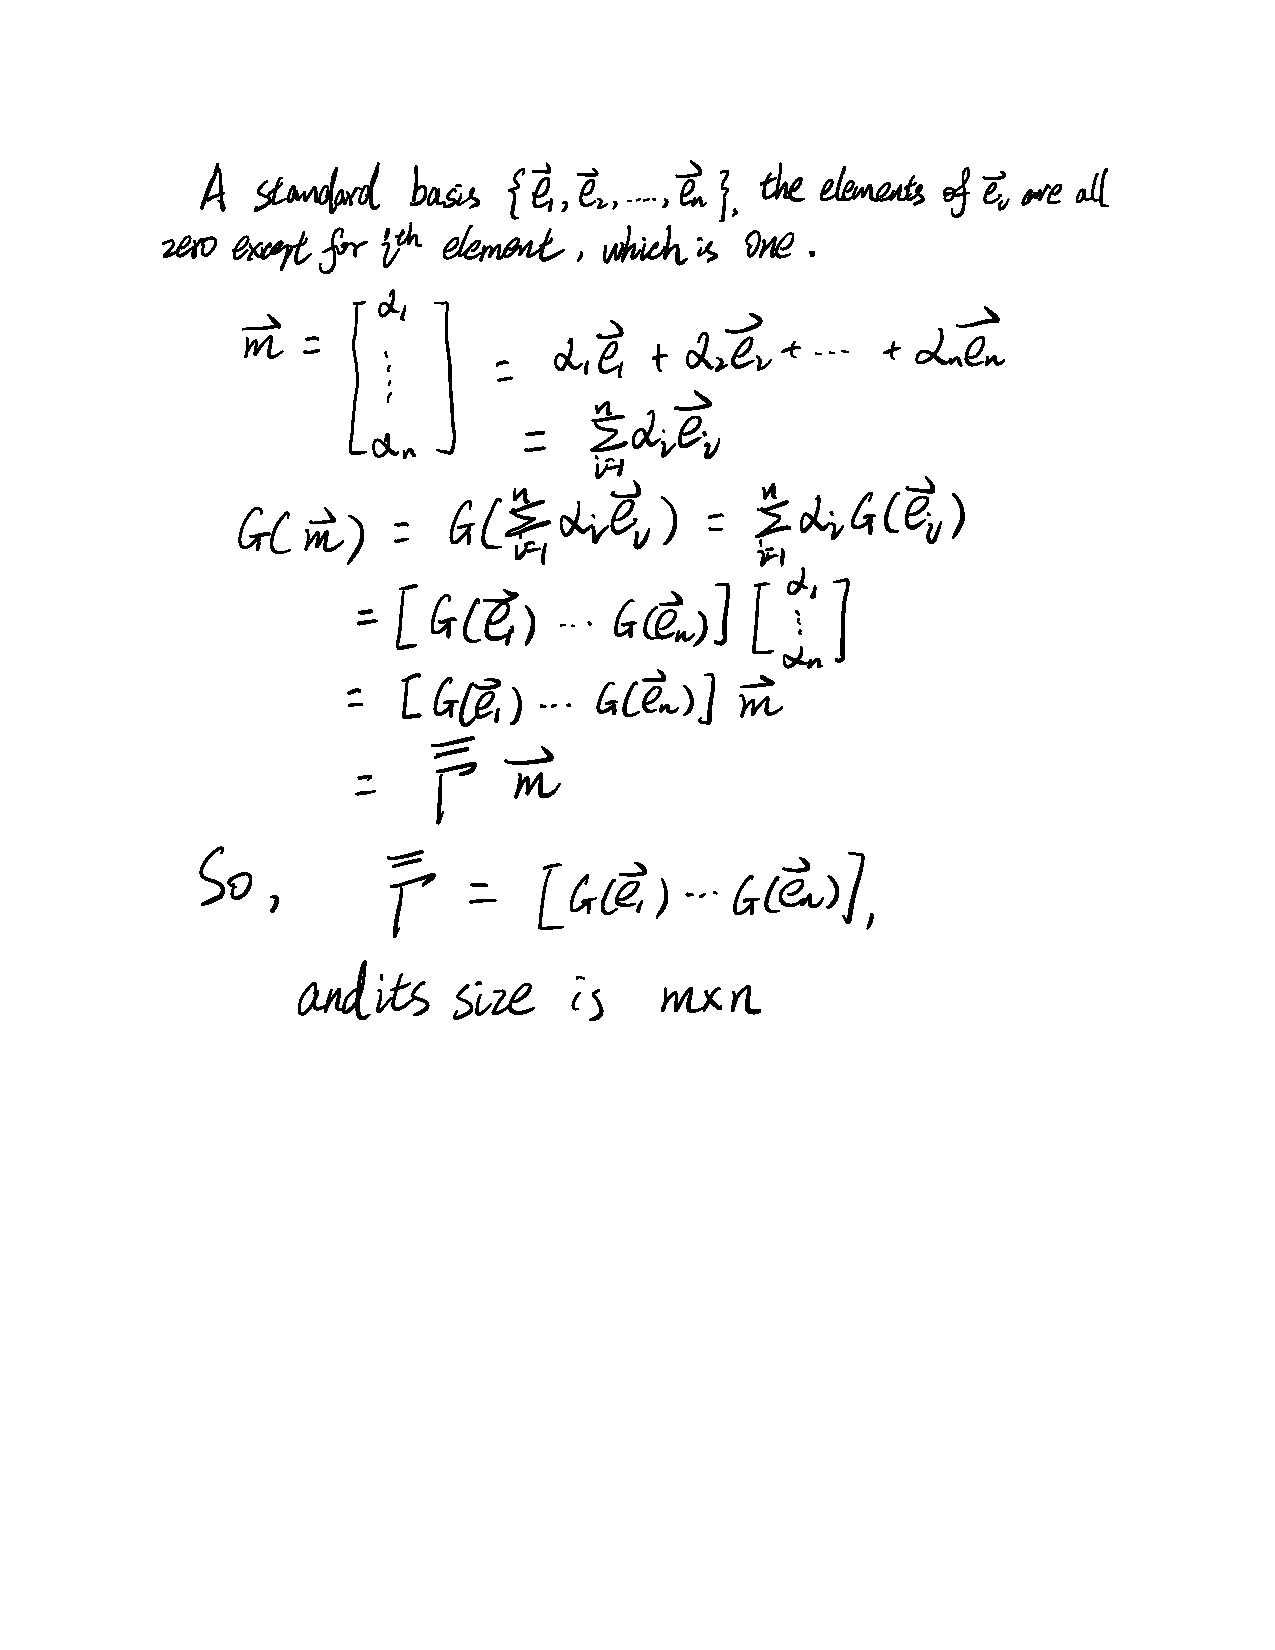
\includegraphics[width=4in, keepaspectratio]{hw2/hw2-1.pdf}
    \label{fig:p1}
\end{figure}


\end{homeworkProblem}

\pagebreak

\begin{homeworkProblem}[2]
Can (1.14) be inconsistent, even with only $m = 3$ data points? How about just $m = 2$
data points? If the system can be inconsistent, give an example. If not, explain why.

\solution

\begin{figure}[htb]
    \centering
    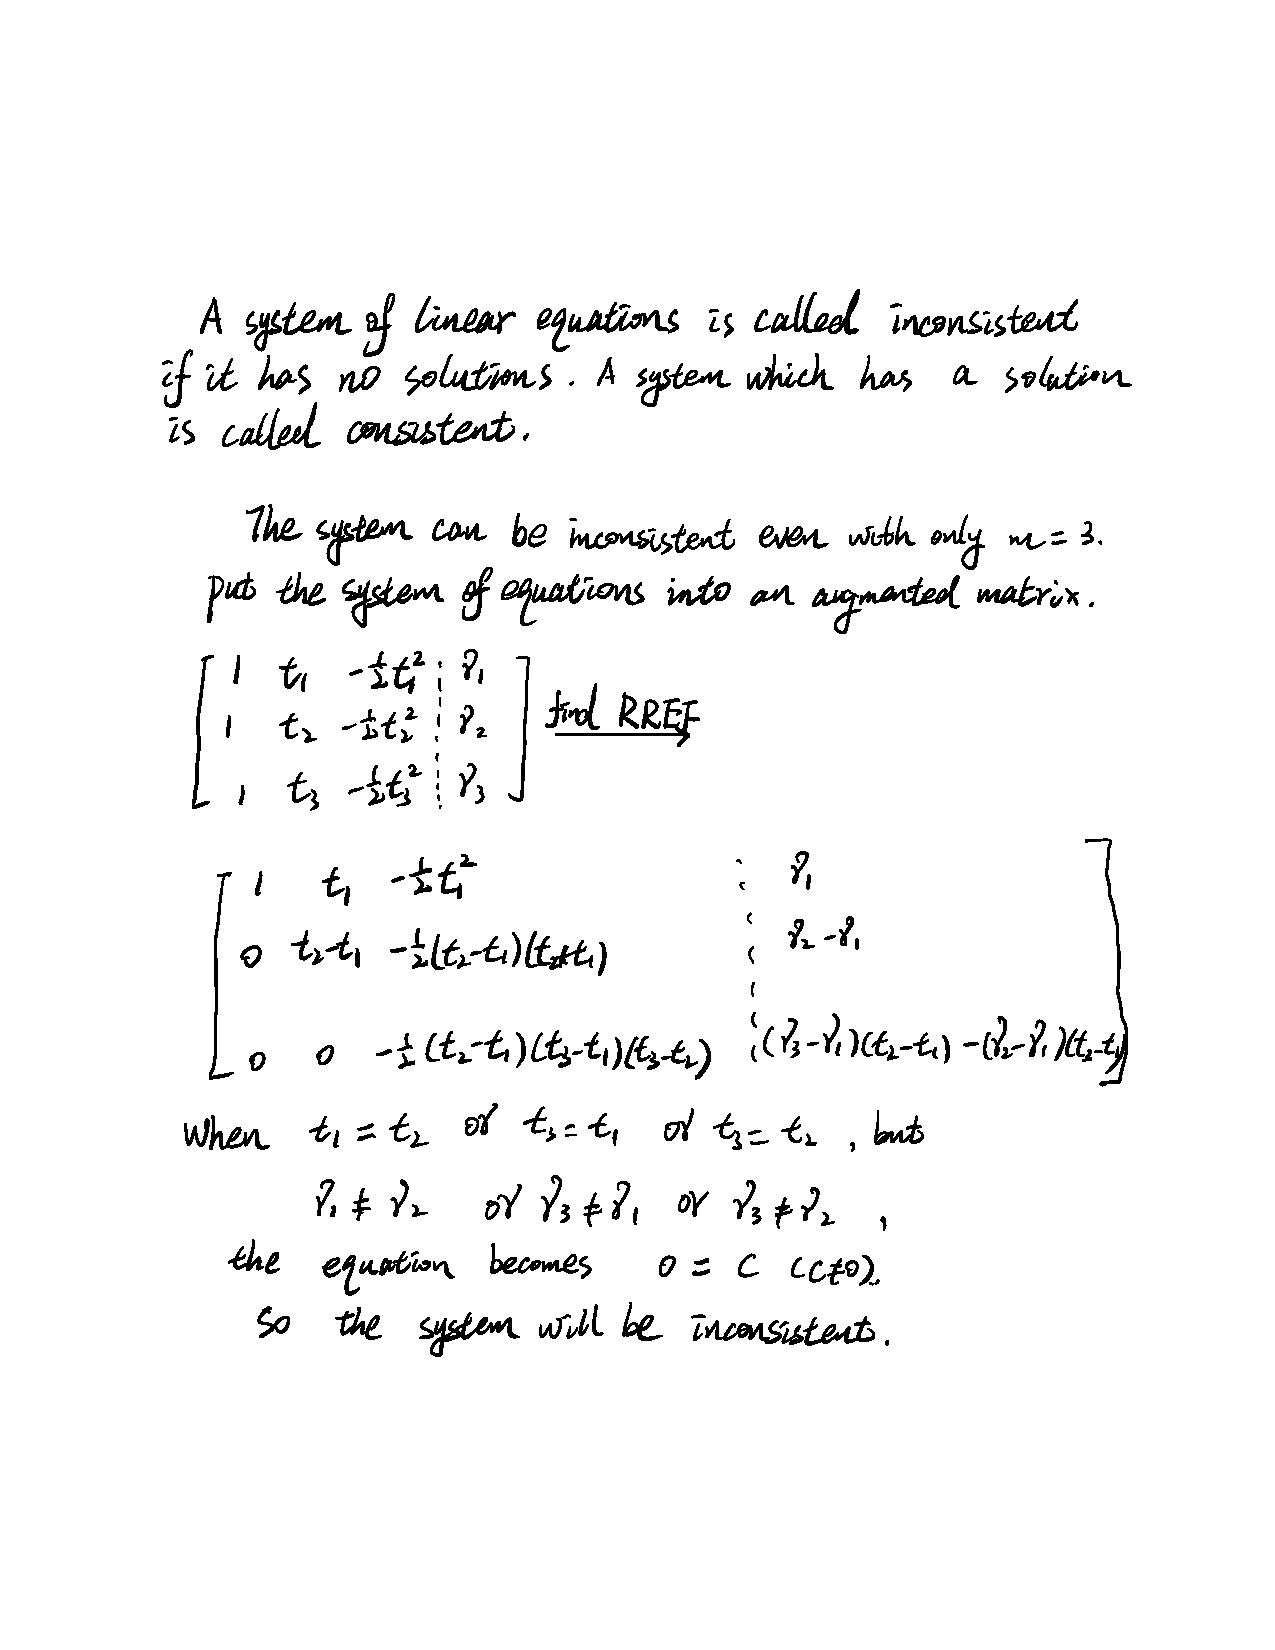
\includegraphics[width=4in, keepaspectratio]{hw2/hw2-2-1.pdf}
    \label{fig:p1}
\end{figure}

\begin{figure}[htb]
    \centering
    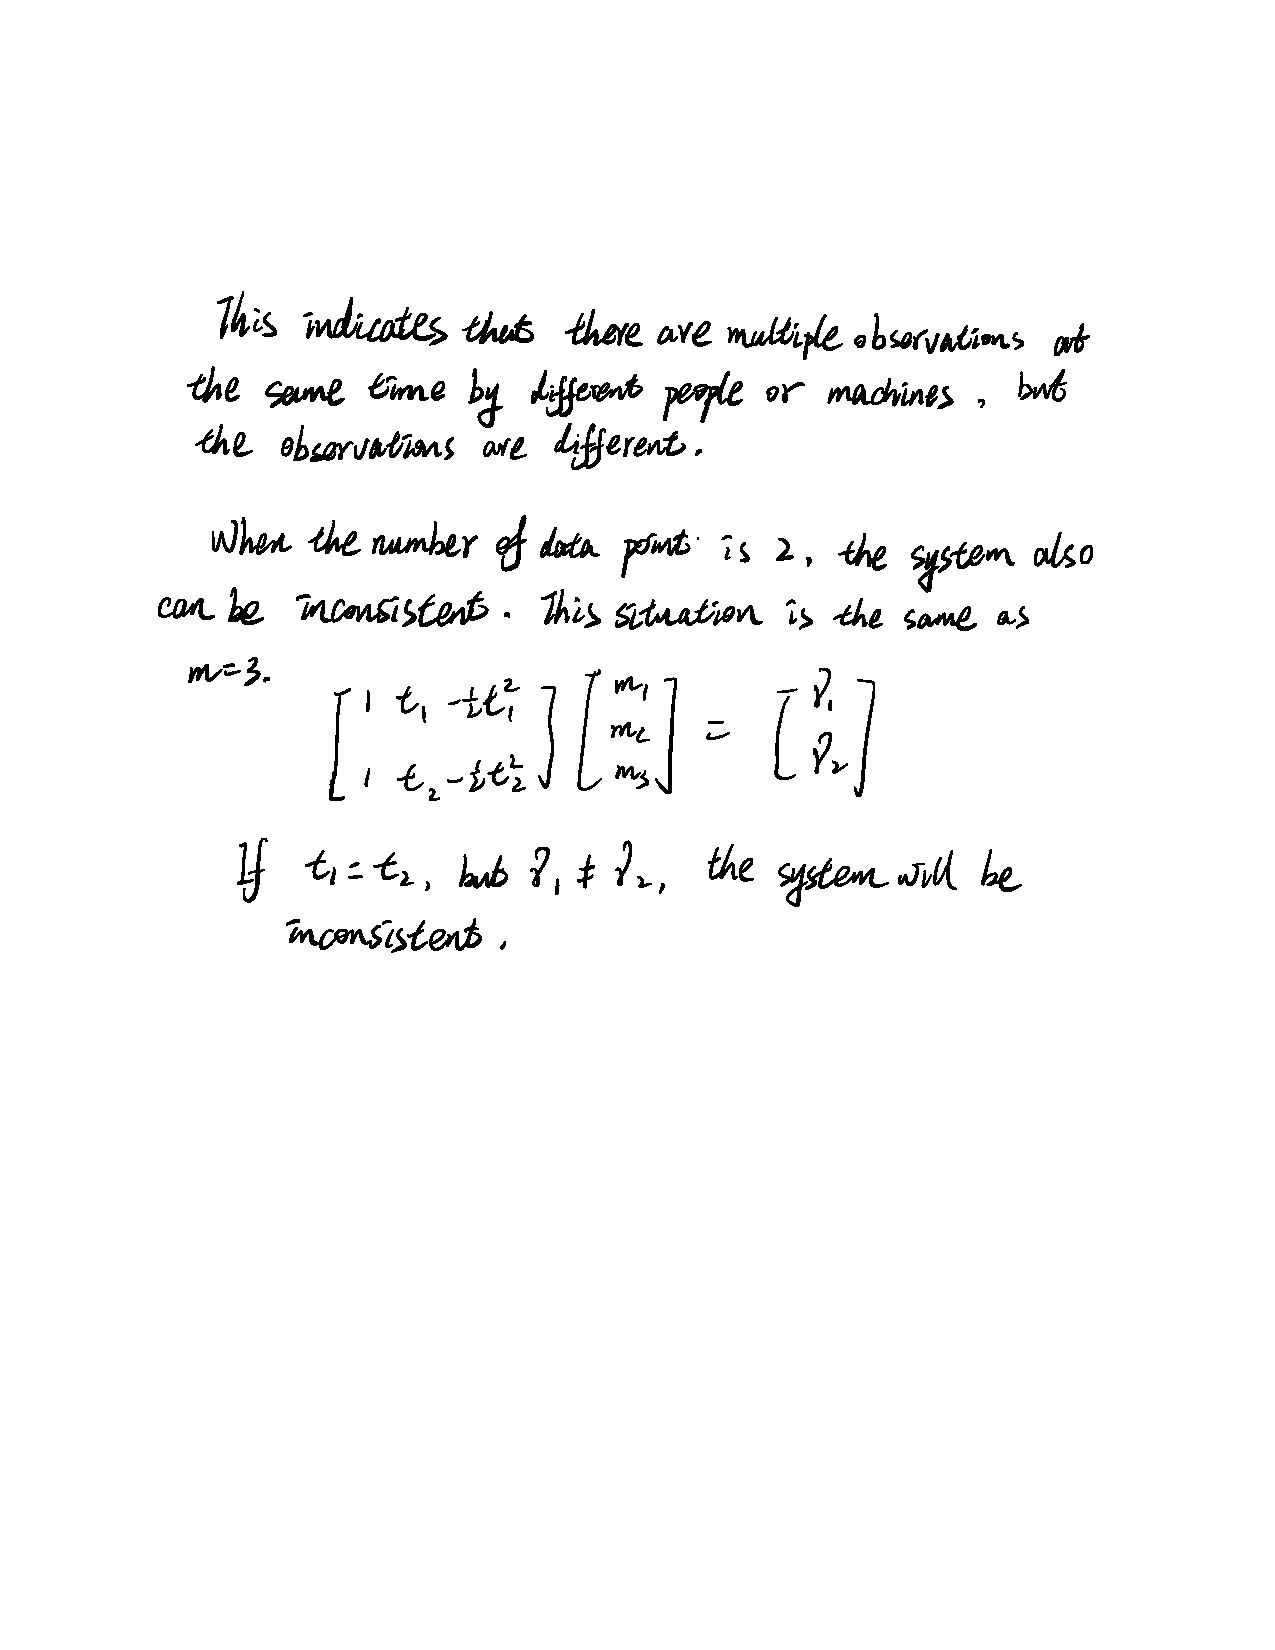
\includegraphics[width=4in, keepaspectratio]{hw2/hw2-2-2.pdf}
    \label{fig:p1}
\end{figure}


\end{homeworkProblem}

\pagebreak

\begin{homeworkProblem}[3]
Consider the borehole vertical seismic profile problem of Examples 1.3 and 1.9 for
$n = 100$ equally spaced seismic sensors located at depths of $z = 0.2, 0.4, ..., 20\ m$,
and for a model $\mathbf{m}$ describing $n$ corresponding equal-length seismic slowness values
for $0.2\ m$ intervals having midpoints at $z - 0.1 m$. \\

\part

Calculate the appropriate system matrix, $\mathbf{G}$, for discretizing the integral equation
(1.21) using the midpoint rule.

\solution

\begin{figure}[htb]
    \centering
    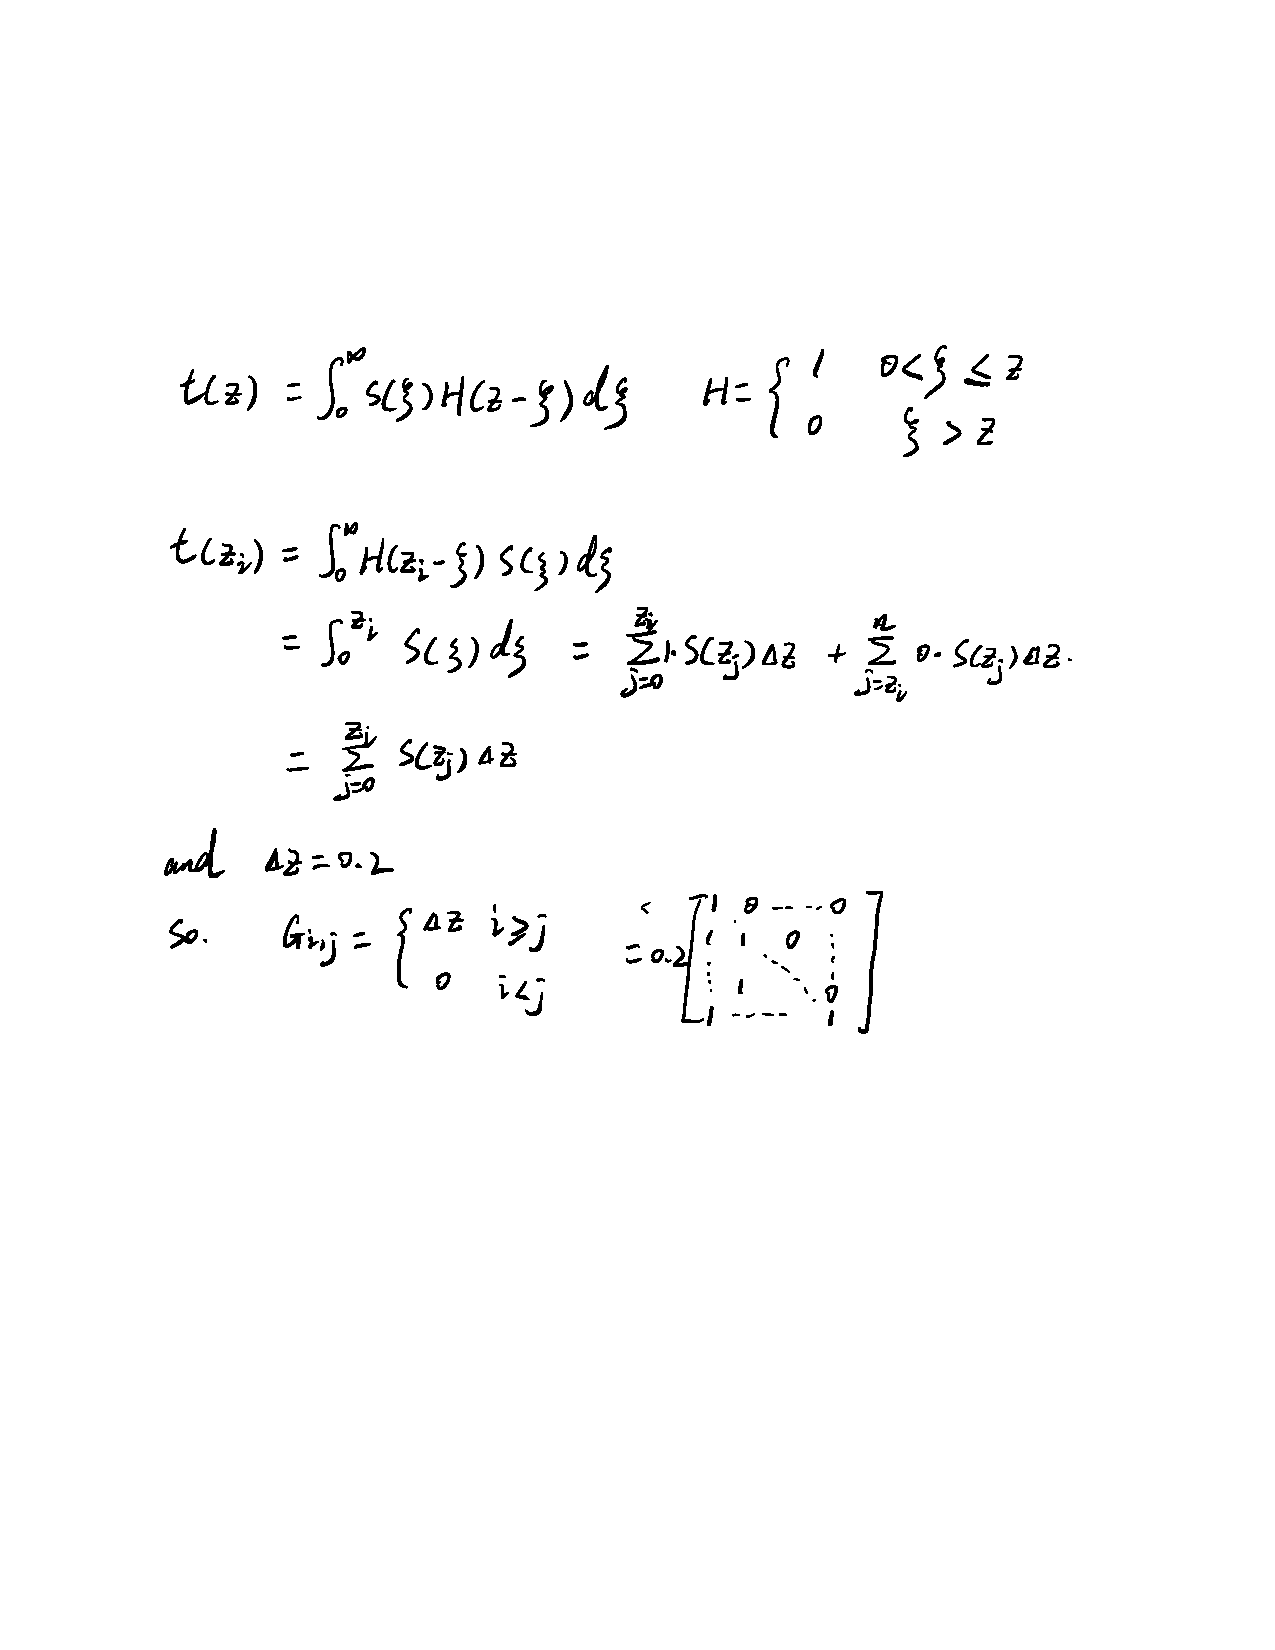
\includegraphics[width=4in, keepaspectratio]{hw2/hw2-3-1.pdf}
    \label{fig:p1}
\end{figure}

\pagebreak

\part

For a seismic velocity model having a linear depth gradient specified by
\begin{equation}
    v=v_{0}+k z ,
\end{equation}
where the velocity at $z=0$ is $v_0 = 1$ km/s and the gradient is $k = 40$ m/s per
m, calculate the true slowness values, $\mathbf{m}_{true}$, at the midpoints of the $n$ intervals.
Integrate the corresponding slowness function for (1.61) using (1.21) to calculate
a noiseless synthetic data vector, $\mathbf{d}$, of predicted seismic travel times at the sensor
depths.

\solution

\begin{figure}[htb]
    \centering
    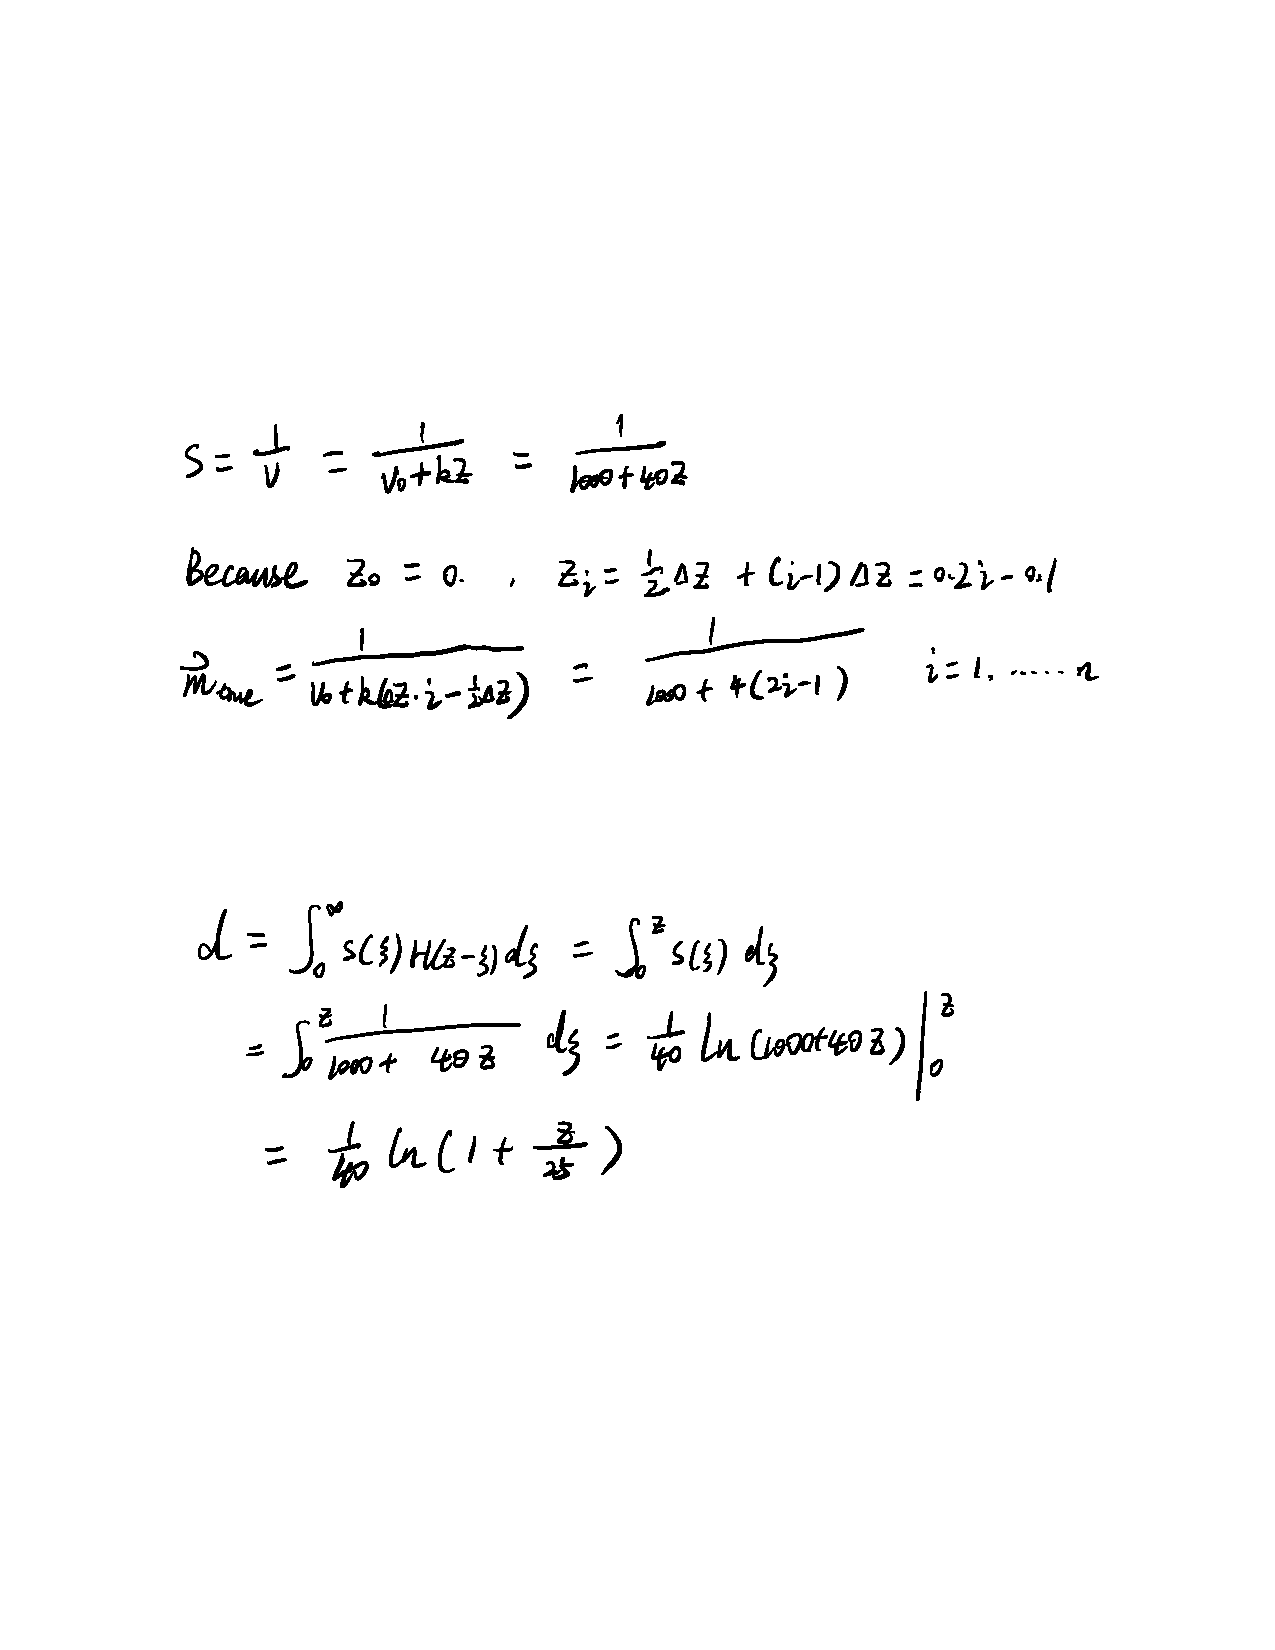
\includegraphics[width=4in, keepaspectratio]{hw2/hw2-3-2.pdf}
    \label{fig:p1}
\end{figure}

\pagebreak

\part

Solve for the slowness, $\mathbf{m}$, as a function of depth using your $\mathbf{G}$ matrix 
and analytically calculated noiseless travel times using the MATLAB backslash operator.
Compare your result graphically with $\mathbf{m}_{true}$.

\solution

\begin{figure}[htb]
    \centering
    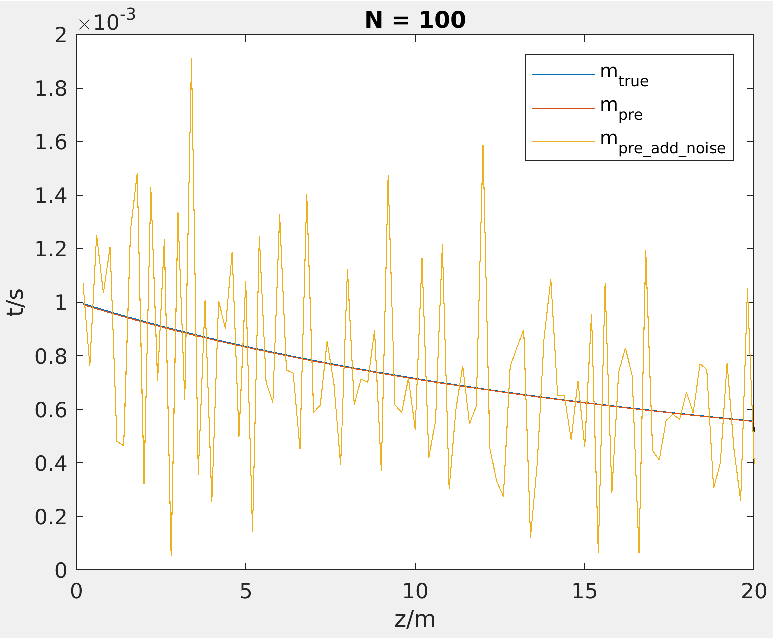
\includegraphics[width=4in, keepaspectratio]{hw2/fig1.pdf}
    \label{fig:p1}
\end{figure}

\begin{figure}[htb]
    \centering
    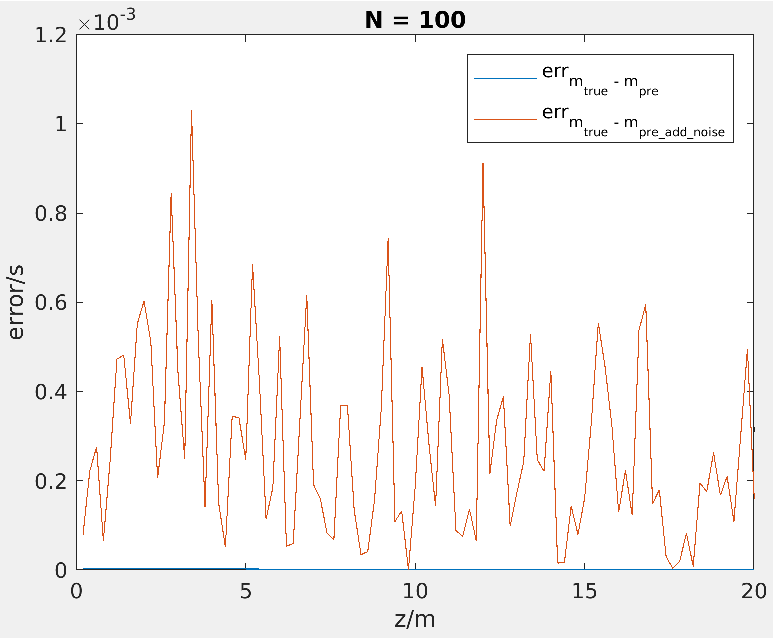
\includegraphics[width=4in, keepaspectratio]{hw2/fig2.pdf}
    \label{fig:p1}
\end{figure}

\pagebreak

\part

Generate a noisy travel time vector where independent normally distributed noise
with a standard deviation of $0.05$ ms is added to the elements of $\mathbf{d}$. Resolve the
system for $\mathbf{m}$ and again compare your result graphically with $\mathbf{m}_{true}$. How has the
model changed?

\solution

The figures are seen in Exercise 3.c (above) 

\begin{figure}[htb]
    \centering
    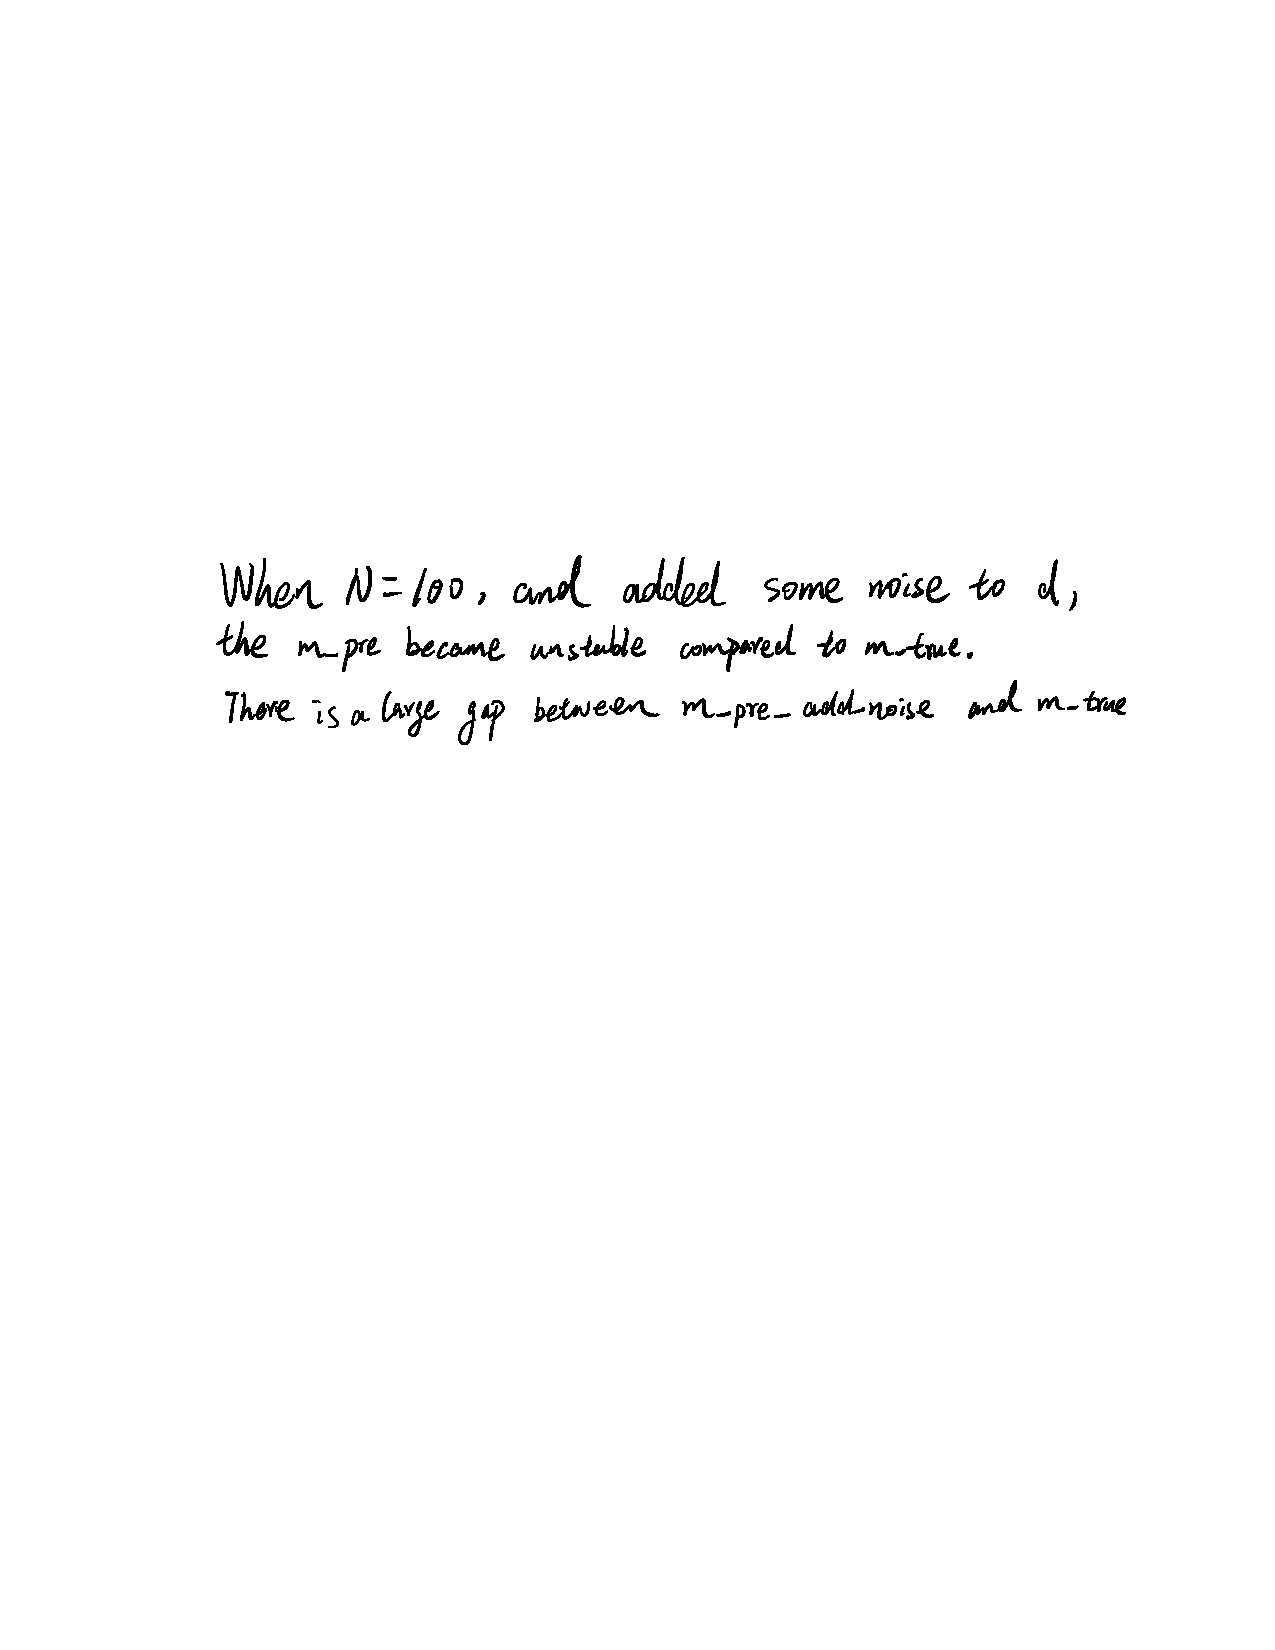
\includegraphics[width=4in, keepaspectratio]{hw2/hw2-3-3.pdf}
    \label{fig:p1}
\end{figure}

\pagebreak

\part

Repeat the problem, but for just $n = 4$ sensor depths and corresponding equal
length slowness intervals. Is the recovery of the true model improved? Explain in
terms of the condition numbers of your $\mathbf{G}$ matrices.

\solution

\begin{figure}[htb]
    \centering
    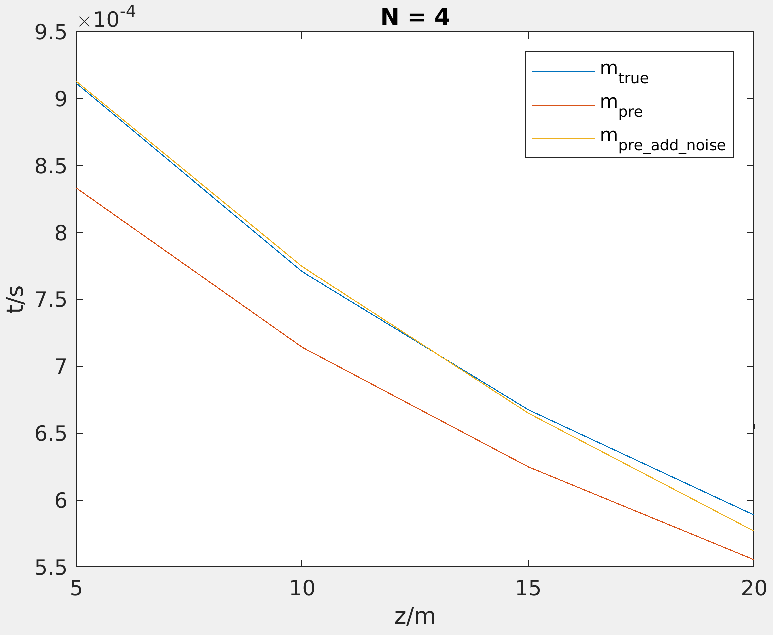
\includegraphics[width=4in, keepaspectratio]{hw2/fig3.pdf}
    \label{fig:p1}
\end{figure}

\begin{figure}[htb]
    \centering
    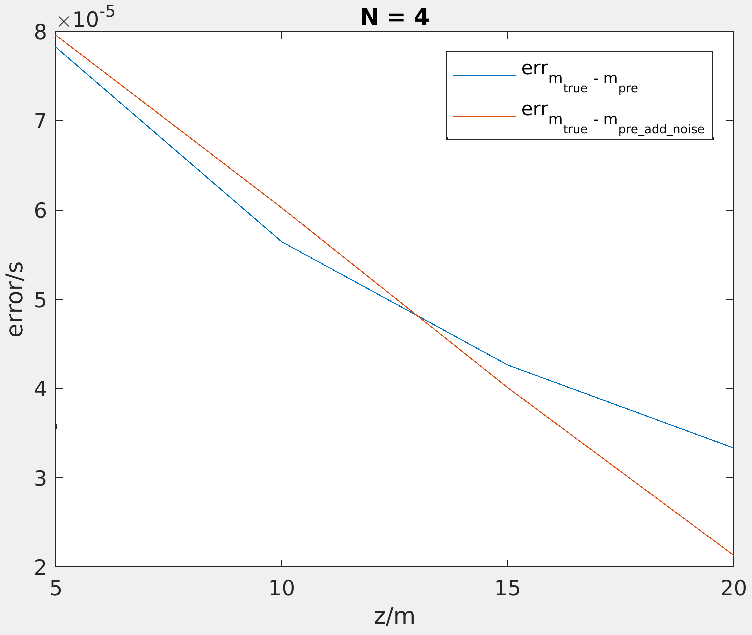
\includegraphics[width=4in, keepaspectratio]{hw2/fig4.pdf}
    \label{fig:p1}
\end{figure}

\begin{figure}[htb]
    \centering
    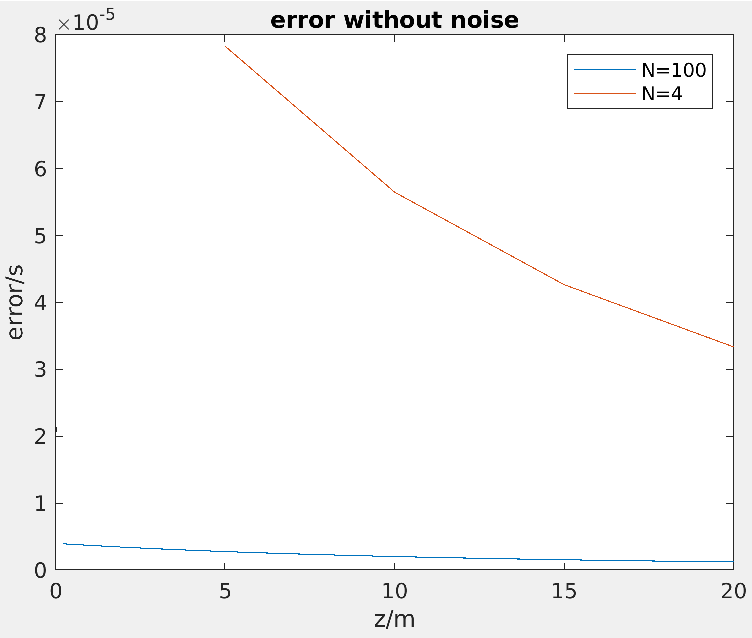
\includegraphics[width=4in, keepaspectratio]{hw2/fig5.pdf}
    \label{fig:p1}
\end{figure}

\begin{figure}[htb]
    \centering
    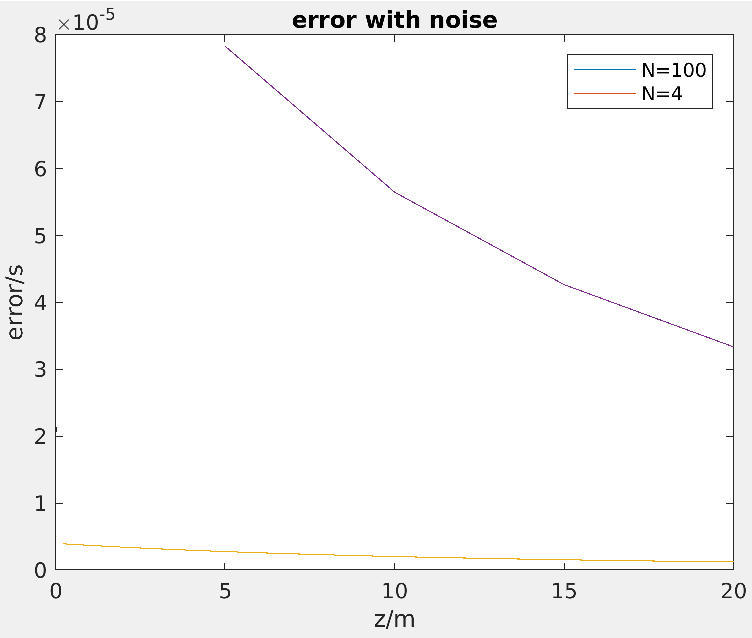
\includegraphics[width=4in, keepaspectratio]{hw2/fig6.pdf}
    \label{fig:p1}
\end{figure}

\begin{figure}[htb]
    \centering
    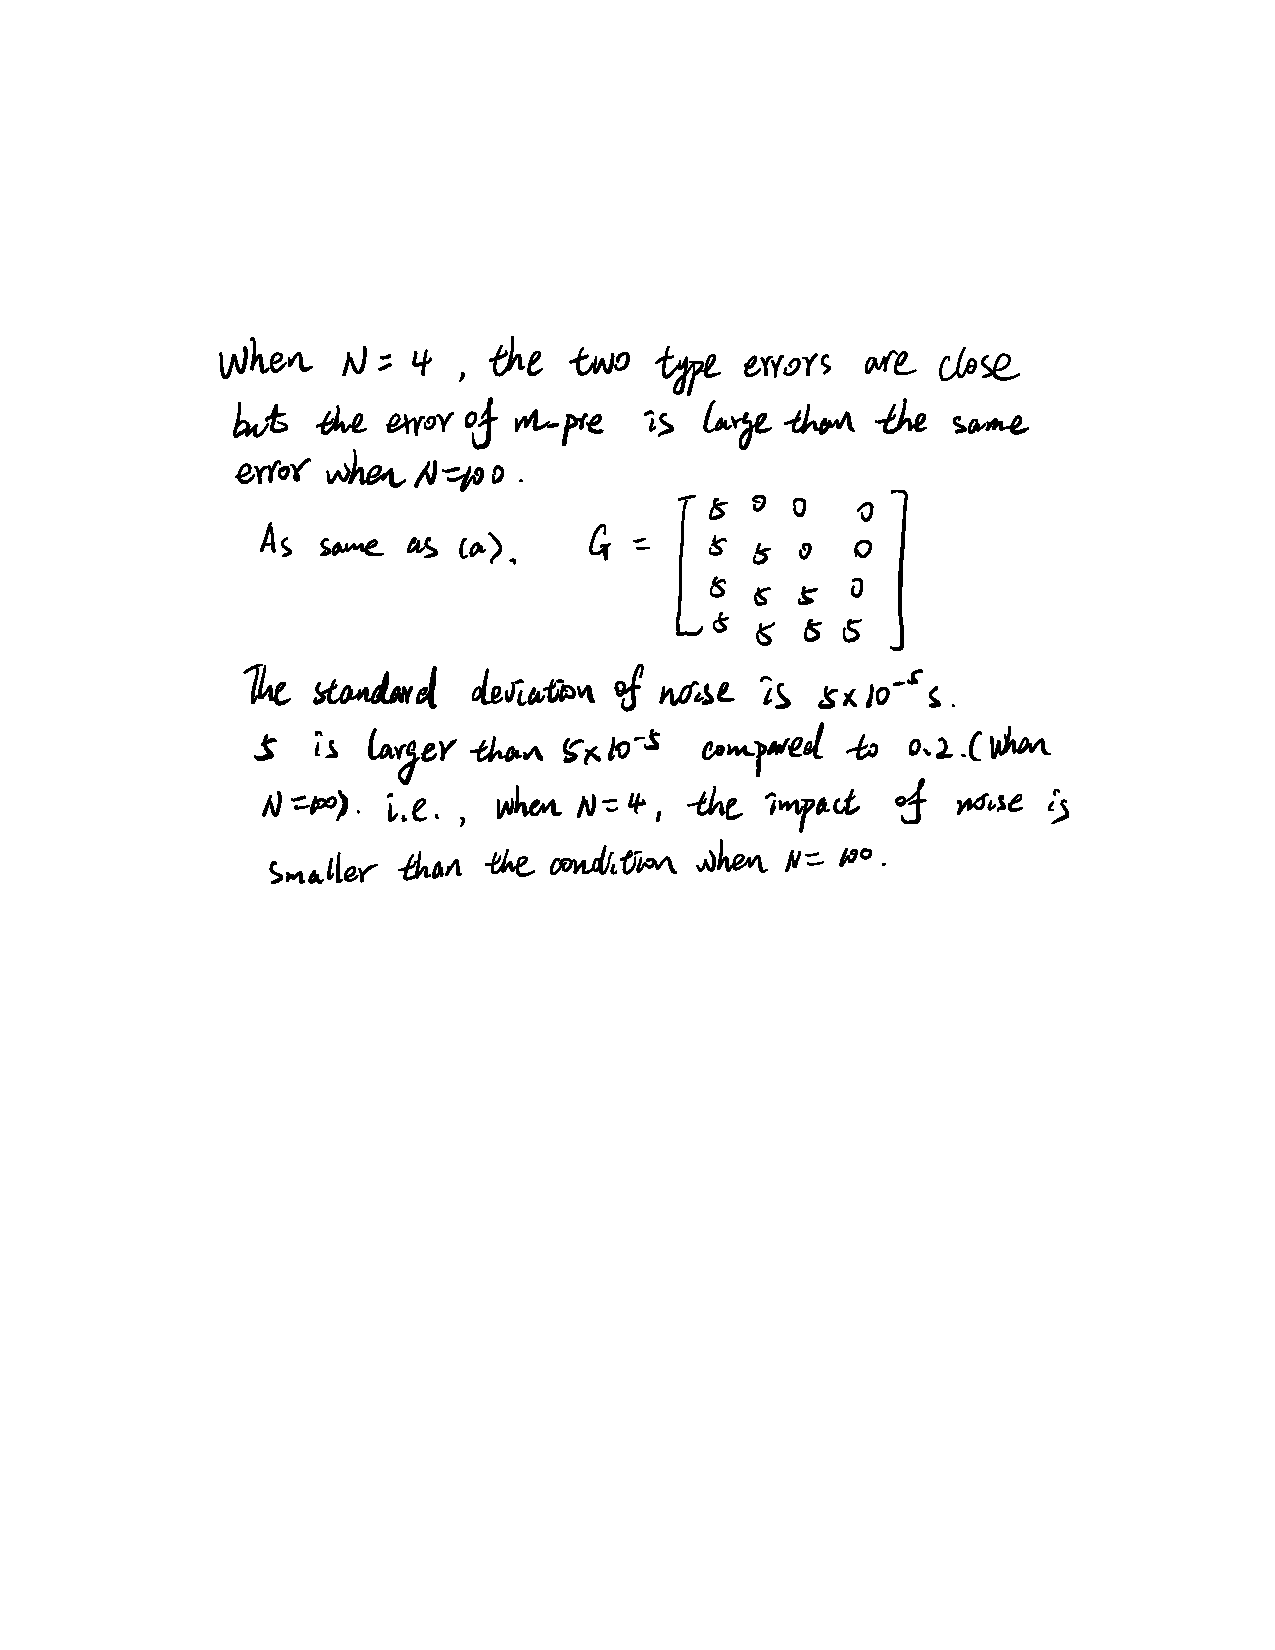
\includegraphics[width=4in, keepaspectratio]{hw2/hw2-3-4.pdf}
    \label{fig:p1}
\end{figure}

\end{homeworkProblem}


\end{document}
